\documentclass[11pt,a4paper]{article}

\usepackage[margin=18mm,top=20mm,bottom=20mm]{geometry}
\usepackage[T1]{fontenc}
\usepackage{lmodern}
\usepackage{graphicx}
\usepackage{booktabs}
\usepackage{tabularx}
\usepackage{array}
\usepackage{amsmath}
\usepackage{xcolor}
\usepackage{enumitem}
\usepackage{listings}
\usepackage{tikz}
\usetikzlibrary{arrows.meta,positioning,fit,shapes.geometric,calc}
\usepackage[hidelinks]{hyperref}

\definecolor{navy}{HTML}{183153}
\definecolor{blue}{HTML}{2C6EAD}
\definecolor{lightblue}{HTML}{EAF3FA}
\definecolor{lightgray}{HTML}{F4F5F7}
\definecolor{green}{HTML}{287D4F}
\definecolor{red}{HTML}{A33B3B}

\hypersetup{
  pdftitle={DSD Final Project Report - Group 1},
  pdfauthor={Group 1: B12901008, B12901137}
}
\pagestyle{plain}
\setlist{nosep,leftmargin=1.5em}
\setlength{\parindent}{0pt}
\setlength{\parskip}{5pt}
\setlength{\emergencystretch}{3em}
\renewcommand{\arraystretch}{1.12}
\providecommand{\micro}{\mu}
\newcommand{\SI}[2]{\ensuremath{#1\,\mathrm{#2}}}

\lstset{
  basicstyle=\ttfamily\small,
  backgroundcolor=\color{lightgray},
  frame=single,
  rulecolor=\color{gray!35},
  columns=fullflexible,
  breaklines=true,
  showstringspaces=false,
  keywordstyle=\color{blue}\bfseries,
  commentstyle=\color{green}
}

\newcommand{\metric}[2]{%
  \begin{minipage}[t]{0.23\linewidth}
    \centering\colorbox{lightblue}{\parbox[c][14mm][c]{0.93\linewidth}{\centering
      {\Large\bfseries\color{navy}#1}\\[-1mm]{\small #2}}}
  \end{minipage}}

\begin{document}
\hypersetup{pageanchor=false}

\begin{titlepage}
  \centering
  \vspace*{18mm}
  {\sffamily\bfseries\color{navy}\fontsize{30}{36}\selectfont
    Hardware Implementation of a\\[2mm]
    Pipelined RISC-V Processor\par}
  \vspace{8mm}
  {\sffamily\Large Digital System Design Final Project Report\par}
  \vspace{15mm}

  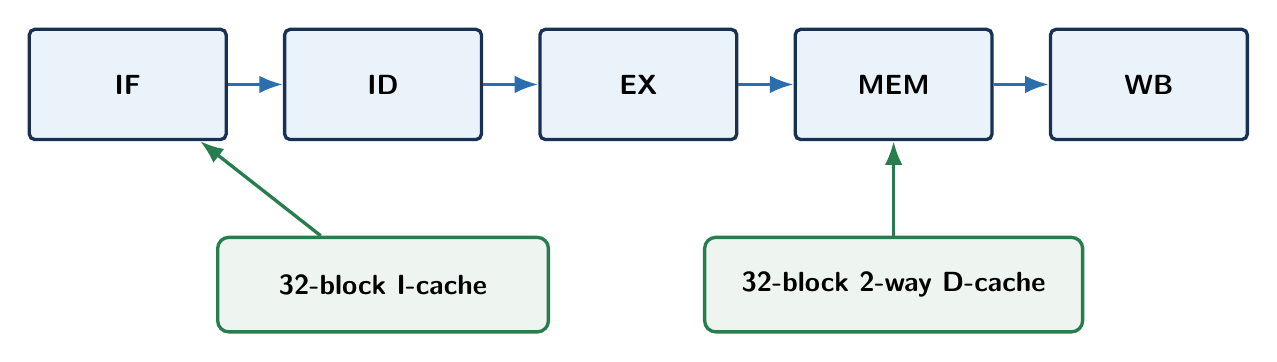
\begin{tikzpicture}[
    stage/.style={draw=navy,very thick,rounded corners=2pt,minimum width=25mm,
                  minimum height=14mm,fill=lightblue,font=\sffamily\bfseries},
    arr/.style={-{Latex[length=3mm]},very thick,color=blue}
  ]
    \node[stage] (if) {IF};
    \node[stage,right=7mm of if] (id) {ID};
    \node[stage,right=7mm of id] (ex) {EX};
    \node[stage,right=7mm of ex] (mem) {MEM};
    \node[stage,right=7mm of mem] (wb) {WB};
    \draw[arr] (if)--(id);
    \draw[arr] (id)--(ex);
    \draw[arr] (ex)--(mem);
    \draw[arr] (mem)--(wb);
    \node[draw=green,very thick,rounded corners,fill=green!8,below=12mm of id,
          minimum width=42mm,minimum height=12mm,font=\sffamily\bfseries] (ic)
          {32-block I-cache};
    \node[draw=green,very thick,rounded corners,fill=green!8,below=12mm of mem,
          minimum width=48mm,minimum height=12mm,font=\sffamily\bfseries] (dc)
          {32-block 2-way D-cache};
    \draw[arr,color=green] (ic)--(if);
    \draw[arr,color=green] (dc)--(mem);
  \end{tikzpicture}

  \vfill
  \begin{tabular}{rl}
    \textbf{Group} & 1\\
    \textbf{Members} & B12901008, B12901137\\
    \textbf{Course} & Digital System Design\\
    \textbf{Date} & June 14, 2026
  \end{tabular}
  \vfill
  {\small National Taiwan University\par}
\end{titlepage}
\hypersetup{pageanchor=true}
\pagenumbering{roman}

\section*{Abstract}
This project implements a synthesizable pipelined RV32 processor that operates
correctly with fast, fixed-latency, and random-latency external memories.  The
processor contains a five-stage core, complete forwarding and stall control,
separate blocking instruction and data caches, and a write-back flush mechanism.
Three extension topics were explored: compressed instructions, multiplication,
and branch prediction.  The final implementation supports the required RV32I
subset, sixteen RV32C compressed instructions, and a multicycle \texttt{MUL}.
We also move unconditional JAL resolution from EX to ID and use a dedicated JAL
immediate path to reduce its control penalty without extending the main EX path.

The submitted gate-level design runs at a \SI{2.7}{ns} testbench clock period
with a synthesized cell area of \SI{769950.83}{\micro m^2}.  Its measured
gate-level times are \SI{193798.947}{ns}, \SI{34423.347}{ns}, and
\SI{722164.647}{ns} for QSort, Conv, and LFSR\_HIST, respectively, yielding the
official area--time product of \(3.7094\times10^{21}\).

\vspace{4mm}
\noindent
\metric{2.7 ns}{Gate clock}\hfill
\metric{769,951}{Cell area (\(\mu m^2\))}\hfill
\metric{RV32I+C+M}{ISA support}\hfill
\metric{3.7094e21}{Final score}

\setcounter{tocdepth}{1}
\tableofcontents
\clearpage
\pagenumbering{arabic}

\section{Specification and Design Goals}

\subsection{Required behavior}
The project specification requires a pipelined RISC-V processor with at least
five stages, synchronous active-low reset, and the prescribed RV32I subset:
integer arithmetic and logic, shifts, comparison, conditional branches,
JAL/JALR, LW/SW, NOP, and the project-specific FLUSH instruction.  The design
must resolve structural, data, and control hazards using hardware forwarding
and stall logic rather than software-inserted NOPs.

Instruction and data memories are external to \texttt{CHIP}.  Correctness is
required under \texttt{fast\_memory}, \texttt{slow\_memory}, and
\texttt{slow\_memory\_random\_latency}.  The latter has long variable latency,
so cache behavior and request stability dominate performance and correctness.
When the final FLUSH instruction retires, all dirty cache lines must have been
written back before \texttt{o\_done} is asserted.

\subsection{Evaluation targets}
The timing target is a post-synthesis testbench clock period below
\SI{3.5}{ns}, no negative setup or hold slack, and no gate-level timing
violation.  Final performance is evaluated by
\[
  \text{Score} =
  A \times T_{\text{QSort}} \times T_{\text{Conv}} \times T_{\text{LFSR\_HIST}},
\]
where lower area and lower simulation time are preferred.  The extension
evaluation additionally checks branch prediction, compressed instructions, and
multiplication at gate level.

\section{Processor Architecture}

\subsection{Top-level organization}
The top-level \texttt{CHIP} contains one pipelined core, a read-only I-cache,
and a write-back D-cache.  Both caches communicate with independent 128-bit
external memory ports.  The final RTL parameters and instantiated cache modules
are shown in Table~\ref{tab:final-config}.

\begin{table}[h]
\centering
\caption{Final implementation configuration.}
\label{tab:final-config}
\begin{tabular}{lll}
\toprule
Component & Final configuration & Purpose\\
\midrule
Core & Five-stage in-order RV32 & Simple, verifiable pipeline\\
I-cache & 32 blocks, direct-mapped & Remove repeated instruction misses\\
D-cache & 32 blocks, 2-way, write-back & Reduce data conflict misses\\
Cache line & 128 bits (four words) & Match external memory interface\\
MUL & Two-cycle multicycle path & Meet timing without a long EX path\\
Control prediction & Always not taken & Lowest hardware cost\\
JAL resolution & ID stage & One-cycle JAL penalty\\
\bottomrule
\end{tabular}
\end{table}

\begin{figure}[h]
\centering
\resizebox{\linewidth}{!}{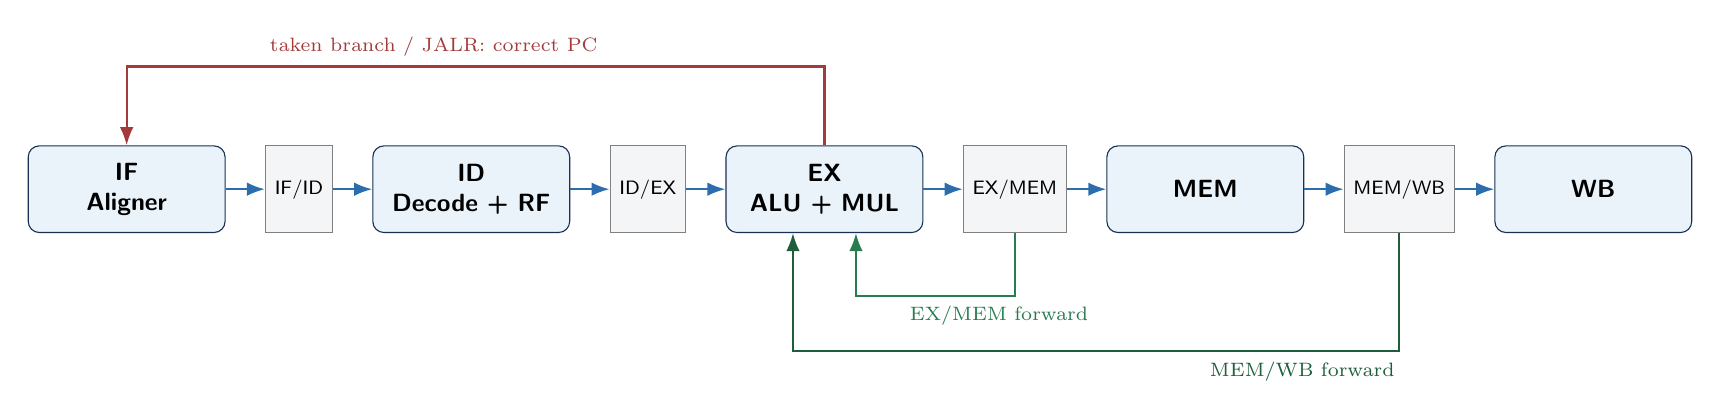
\begin{tikzpicture}[
  node distance=5mm and 5mm,
  block/.style={draw=navy,rounded corners,fill=lightblue,minimum width=25mm,
                minimum height=11mm,align=center,font=\small\sffamily\bfseries},
  reg/.style={draw=gray,fill=lightgray,minimum width=8mm,minimum height=11mm,
              font=\scriptsize\sffamily},
  arr/.style={-{Latex[length=2.3mm]},thick,color=blue}
]
  \node[block] (if) {IF\\Aligner};
  \node[reg,right=of if] (r1) {IF/ID};
  \node[block,right=of r1] (id) {ID\\Decode + RF};
  \node[reg,right=of id] (r2) {ID/EX};
  \node[block,right=of r2] (ex) {EX\\ALU + MUL};
  \node[reg,right=of ex] (r3) {EX/MEM};
  \node[block,right=of r3] (mem) {MEM};
  \node[reg,right=of mem] (r4) {MEM/WB};
  \node[block,right=of r4] (wb) {WB};
  \foreach \a/\b in {if/r1,r1/id,id/r2,r2/ex,ex/r3,r3/mem,mem/r4,r4/wb}
    \draw[arr] (\a)--(\b);
  \coordinate (redirectTop) at ($(ex.north)+(0,10mm)$);
  \draw[arr,red] (ex.north) -- (redirectTop)
    -| node[pos=0.28,above,font=\scriptsize]{taken branch / JALR: correct PC} (if.north);
  \coordinate (exFwdNear) at ($(ex.south)+(4mm,0)$);
  \coordinate (exFwdFar) at ($(ex.south)+(-4mm,0)$);
  \coordinate (fwdNear) at ($(exFwdNear)+(0,-8mm)$);
  \coordinate (fwdFar) at ($(exFwdFar)+(0,-15mm)$);
  \draw[arr,green] (r3.south) |- node[pos=0.55,below,font=\scriptsize]{EX/MEM forward}
    (fwdNear) -- (exFwdNear);
  \draw[arr,green!75!black] (r4.south) |- node[pos=0.58,below,font=\scriptsize]{MEM/WB forward}
    (fwdFar) -- (exFwdFar);
\end{tikzpicture}}
\caption{Core pipeline and major feedback paths.}
\end{figure}

\subsection{Pipeline operation}
The IF stage fetches and aligns either a 16-bit or 32-bit instruction.  ID
decodes the instruction, reads the register file, generates immediates, and
resolves JAL.  EX performs ALU operations, branch comparison, JALR target
generation, forwarding selection, and multicycle multiplication.  MEM issues
load/store requests through the D-cache, while WB commits the selected result
to the register file.

Each stage carries a \texttt{valid} bit and only valid instructions may cause
architectural side effects.  This makes bubbles and flushes explicit and avoids
depending on arbitrary payload values after reset.  The pipeline is globally
held while an outstanding memory transaction is incomplete.  During a MUL
stall, earlier instructions are allowed to drain while younger stages are held.

\section{Hazards and Control Flow}

\subsection{Data and structural hazards}
EX operands pass through two forwarding multiplexers.  An ALU result can be
forwarded from EX/MEM; a completed ALU or load result can be forwarded from
MEM/WB.  The same forwarded second operand is used as store data, preventing a
common store-after-produce failure.  Loads require one bubble when the following
instruction consumes the destination because load data is not available at the
start of the next EX cycle.

The separate I-cache and D-cache eliminate contention between instruction fetch
and data access.  A cache miss still creates a structural dependency on its
external memory port.  The core therefore keeps requests and addresses stable
and stalls until the corresponding \texttt{mem\_ready} is observed.

\begin{table}[h]
\centering
\caption{Hazard handling summary.}
\begin{tabularx}{\linewidth}{lXl}
\toprule
Hazard & Detection or mechanism & Action\\
\midrule
EX/MEM RAW & Destination matches EX source; result is not a load & Forward\\
MEM/WB RAW & Destination matches EX source & Forward\\
Store-data RAW & Destination matches store's second source & Forward\\
Load-use & ID/EX load destination matches IF/ID source & Insert bubble\\
Memory wait & Active memory request without ready & Hold pipeline\\
MUL wait & Valid MUL has not completed & Hold younger stages\\
Taken branch/JALR & EX redirect is valid & Flush younger instructions\\
JAL & Decode detects valid JAL & Redirect in ID, flush IF only\\
\bottomrule
\end{tabularx}
\end{table}

\subsection{Control hazards and ID-stage JAL}
The baseline control policy is always not taken.  Conditional branches and
JALR are resolved in EX because they require forwarded register operands.
Incorrectly fetched younger instructions are invalidated when EX redirects the
PC.

JAL does not require register operands.  We therefore move its target
calculation to ID, reducing its penalty from two flushed instructions to one.
A dedicated immediate concatenation computes the J-type offset directly from
instruction bits, bypassing the general immediate multiplexer:
\[
\texttt{jal\_target} = \texttt{ifid\_pc} +
\{\!\{\texttt{inst[31]}\}\!,\texttt{inst[19:12]},\texttt{inst[20]},
\texttt{inst[30:21]},0\}.
\]
Branches and JALR remain in EX because moving their forwarding and comparison
logic to ID would threaten the clock period.

\section{Cache Design and Optimization}

\subsection{Cache microarchitecture}
The I-cache is a direct-mapped read-only blocking cache.  The D-cache is a
two-way set-associative blocking cache with valid and dirty bits.  On a dirty
miss, the old 128-bit line is written back before the requested line is
refilled.  Word selection occurs inside the cached line.  The D-cache
replacement policy selects a way within the indexed set, and the FLUSH FSM
walks through every set and way, writing back all dirty lines.

The core's done flag and the D-cache flush-done flag are combined at the top
level.  Consequently, \texttt{o\_done} cannot become high before architectural
execution is complete and memory is coherent with the golden checker.

\subsection{Cache sweep methodology}
Before committing to RTL configurations, we built a C++ instruction-set and
cache simulator that reads the supplied patterns.  It counts instruction/data
accesses, misses, writebacks, and expected slow-memory delay for several block
counts and associativities.  Promising cases were then tested in RTL because
the analytical model cannot capture synthesized area, critical paths, or
pipeline-control overhead.

\begin{table}[h]
\centering
\caption{Selected cache miss-rate observations from the software sweep.}
\label{tab:cache-sweep}
\begin{tabular}{llrrr}
\toprule
Pattern & Cache & 16 blocks, 1-way & 32 blocks, 1-way & 64 blocks, 1-way\\
\midrule
QSort & I miss rate & 2.5498\% & 0.0541\% & 0.0541\%\\
QSort & D miss rate & 6.7210\% & 3.8209\% & 1.7041\%\\
Conv & I miss rate & 3.6880\% & 0.9164\% & 0.8941\%\\
Conv & D miss rate & 21.2606\% & 2.9163\% & 2.9163\%\\
LFSR\_HIST & I miss rate & 18.4577\% & 0.0130\% & 0.0130\%\\
LFSR\_HIST & D miss rate & 37.5730\% & 36.5347\% & 35.4964\%\\
\bottomrule
\end{tabular}
\end{table}

The largest gain is obtained by increasing the I-cache from 16 to 32 blocks:
LFSR\_HIST's instruction miss rate collapses from 18.46\% to 0.013\%.  A larger
two-way D-cache substantially helps QSort and Conv, while LFSR\_HIST remains
dominated by a data access pattern with poor locality.  Balancing area against
miss-rate improvement, the final submitted design uses 32 direct-mapped
I-cache blocks and 32 two-way D-cache blocks.  Higher
associativity was rejected because extra tag comparisons, data multiplexers,
and replacement state provided little additional benefit for the supplied
workloads.

\begin{table}[h]
\centering
\caption{Selected RTL cache experiment cycles (QSort / Conv / LFSR\_HIST).}
\begin{tabular}{lrrr}
\toprule
Configuration & QSort & Conv & LFSR\_HIST\\
\midrule
I16 / D16, both 1-way & 112,201 & 21,300 & 1,226,355\\
I32 / D16, both 1-way & 87,807 & 20,873 & 278,220\\
I32 / D32, both 1-way & 79,718 & 14,678 & 277,771\\
I32 / D64, both 1-way & 73,561 & 10,965 & 277,357\\
\bottomrule
\end{tabular}
\end{table}

\section{ISA Extensions}

\subsection{Compressed instruction support}
The IF stage determines instruction length from the low two bits of the current
halfword.  A compressed instruction is expanded into an equivalent 32-bit
RV32I instruction before decode, allowing the remainder of the pipeline to be
shared.  Sixteen compressed operations are supported:
\texttt{c.nop}, \texttt{c.add}, \texttt{c.mv}, \texttt{c.addi},
\texttt{c.andi}, \texttt{c.slli}, \texttt{c.srli}, \texttt{c.srai},
\texttt{c.sw}, \texttt{c.lw}, \texttt{c.beqz}, \texttt{c.bnez},
\texttt{c.j}, \texttt{c.jal}, \texttt{c.jr}, and \texttt{c.jalr}.

\begin{figure}[h]
\centering
\resizebox{\linewidth}{!}{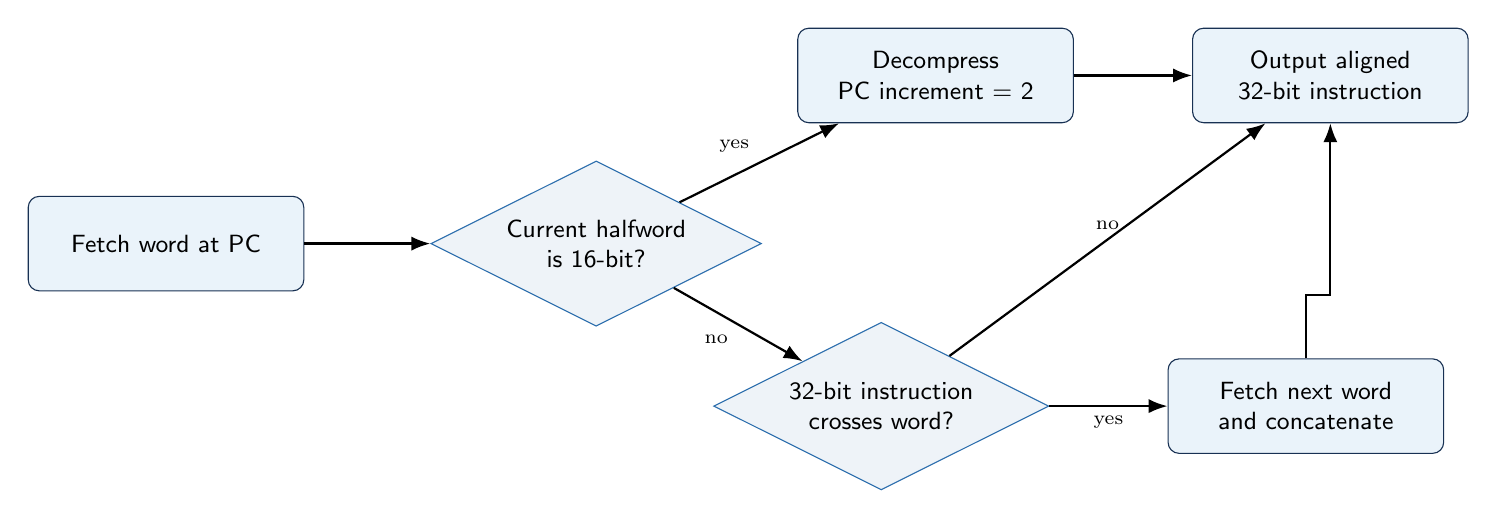
\begin{tikzpicture}[
  s/.style={draw=navy,rounded corners,fill=lightblue,minimum width=35mm,
            minimum height=12mm,align=center,font=\small\sffamily},
  d/.style={diamond,draw=blue,fill=blue!8,aspect=2,align=center,font=\small\sffamily},
  a/.style={-{Latex[length=2.4mm]},thick}
]
  \node[s] (fetch) {Fetch word at PC};
  \node[d,right=16mm of fetch] (low) {Current halfword\\is 16-bit?};
  \node[s,above right=10mm and 15mm of low] (dec) {Decompress\\PC increment = 2};
  \node[d,below right=10mm and 15mm of low] (cross) {32-bit instruction\\crosses word?};
  \node[s,right=15mm of dec] (normal) {Output aligned\\32-bit instruction};
  \node[s,right=15mm of cross] (second) {Fetch next word\\and concatenate};
  \draw[a] (fetch)--(low);
  \draw[a] (low)--node[above left,font=\scriptsize]{yes}(dec);
  \draw[a] (low)--node[below left,font=\scriptsize]{no}(cross);
  \draw[a] (dec)--(normal);
  \draw[a] (cross)--node[above,font=\scriptsize]{no}(normal);
  \draw[a] (cross)--node[below,font=\scriptsize]{yes}(second);
  \coordinate (secondRoute) at ($(second.north)+(0,8mm)$);
  \draw[a] (second.north) -- (secondRoute) -| (normal.south);
\end{tikzpicture}}
\caption{Instruction alignment and decompression flow.}
\end{figure}

If a 32-bit instruction begins in the upper halfword, the aligner saves that
halfword and fetches the next word before concatenation.  This also handles a
cross-cache-line instruction.  The pipeline carries an explicit PC increment
(\(2\) or \(4\)) so that compressed JAL/JALR write the correct link address.
The aligned 32-bit fast path remains single-cycle for normal final patterns.

\subsection{Multicycle multiplication}
A single-cycle combinational multiplier would lengthen EX and make the target
period difficult to achieve.  The implemented unit captures already-forwarded
operands into dedicated registers, computes the product, and captures the
result after a two-cycle multicycle interval.  IF, ID, and the active EX
instruction are held while older EX/MEM and MEM/WB instructions drain.

The synthesis constraints match this microarchitecture:
\begin{lstlisting}[language=tcl]
set mul_cycles 2
set_multicycle_path $mul_cycles -setup \
  -from [get_cells -hier *mul_a_reg*] \
  -to   [get_cells -hier *mul_result_reg*]
set_multicycle_path 1 -hold \
  -from [get_cells -hier *mul_a_reg*] \
  -to   [get_cells -hier *mul_result_reg*]
\end{lstlisting}
The official multiplication gate-level pattern completes in
\SI{738.147}{ns} at a \SI{2.7}{ns} clock period.

\subsection{Branch-prediction exploration}
We evaluated always-not-taken, always-taken, backward-taken/forward-not-taken
(BTFNT), global counters, bimodal tables, and gshare using branch traces from
the supplied workloads.  The specialized BrPred test favors a small bimodal
table, but that improvement does not generalize to the three performance
workloads.  In particular, LFSR\_HIST branches depend strongly on generated
data, so more state does not imply better prediction.

\begin{table}[h]
\centering
\caption{Software branch-prediction accuracy.}
\label{tab:branch}
\begin{tabular}{lrrrr}
\toprule
Method & BrPred & QSort & Conv & LFSR\_HIST\\
\midrule
Always not taken & 37.97\% & 72.44\% & 63.58\% & 85.46\%\\
Always taken & 62.03\% & 27.56\% & 36.42\% & 14.54\%\\
BTFNT & 73.42\% & 72.44\% & 66.05\% & 85.46\%\\
Global 3-bit counter & 68.35\% & 70.48\% & 63.58\% & 85.44\%\\
8-entry 2-bit bimodal & 93.67\% & 74.08\% & 63.58\% & 83.60\%\\
\bottomrule
\end{tabular}
\end{table}

The final core retains always-not-taken because it has zero predictor-table
area, is already strong on QSort and LFSR\_HIST, and avoids adding another
redirect path to IF.  We instead applied the lower-risk ID-stage JAL
optimization.  The final BrPred gate-level result is 558 cycles; the
hasHazard reference pattern takes 2,375 cycles.

\section{Synthesis and Timing Closure}

\subsection{Flow and constraints}
The design is synthesized in Synopsys Design Compiler with the TSMC
\SI{0.13}{\micro m} cell library.  The flow analyzes and elaborates the single
RTL source, applies SDC constraints, runs \texttt{compile\_ultra}, flattens the
design, performs timing-focused incremental optimization, and emits Verilog,
SDF, DDC, SDC, and reports.

The submitted run uses a \SI{2.7}{ns} clock, \SI{0.1}{ns} clock uncertainty,
and \SI{0.5}{ns} clock latency.  External memory inputs and outputs receive
half-cycle maximum delay constraints because the testbench memory interface
operates on the opposite clock phase.  Reset release and multiplication are
explicitly constrained as multicycle paths.

\subsection{Synthesis results}
\begin{table}[h]
\centering
\caption{Final synthesis and timing-closure summary.}
\label{tab:syn}
\begin{tabular}{lr}
\toprule
Metric & Result\\
\midrule
Clock period & \SI{2.70}{ns}\\
Critical path slack / total negative slack & \SI{0.00}{ns} / \SI{0.00}{ns}\\
Setup / hold violating paths & 0 / 0\\
Logic levels on reported CLK critical path & 8\\
Combinational / sequential cell count & 28,294 / 11,595\\
Total cell area & \SI{769950.832599}{\micro m^2}\\
\bottomrule
\end{tabular}
\end{table}

The reported critical path begins at external \texttt{mem\_ready\_D} and ends
at a D-cache data-array enable flip-flop.  It meets timing exactly after
including the \SI{1.35}{ns} external input delay.  This confirms that the cache
control/refill interface, rather than the integer ALU, is the dominant timing
concern.

The final QoR reports zero setup and hold violating paths.  The critical path
is associated with D-cache control rather than the integer ALU, so timing
optimization focused on cache request/refill logic and the external-memory
interface.  The final cell area includes the 32-block direct-mapped I-cache,
32-block two-way D-cache, compressed-instruction aligner/decoder, and
multicycle multiplier.

\section{Verification and Final Results}

\subsection{Verification strategy}
Verification proceeded from isolated behavior to combined regression:
\begin{enumerate}
  \item Validate the required RV32I subset with noHazard and targeted ALU tests.
  \item Exercise EX/MEM forwarding, MEM/WB forwarding, store-data forwarding,
        load-use bubbles, branch forwarding, JAL/JALR redirects, and flushes.
  \item Run all tests against fast, fixed-latency, and random-latency memories.
  \item Validate compressed lower/upper halfwords, cross-word instructions,
        cross-line instructions, and \(PC+2\) compressed links.
  \item Validate MUL with forwarded operands and surrounding memory traffic.
  \item Re-run RTL and post-synthesis gate-level simulations for final patterns.
\end{enumerate}

Small directed patterns were essential because a full hasHazard failure often
appears far after the original bad redirect or forwarded value.  Examples
include adjacent branch dependencies, load-to-branch, store-before-flush,
JALR with negative immediate, and D-cache conflict/flush cases.

\subsection{Official final results}
\begin{table}[h]
\centering
\caption{Submitted gate-level results at a \SI{2.7}{ns} testbench clock.}
\label{tab:results}
\begin{tabular}{llr}
\toprule
Category & Pattern or metric & Result\\
\midrule
Branch/control & BrPred & 558 cycles\\
Branch/control & hasHazard & 2,375 cycles\\
Compressed & Compression simulation time & \SI{1874.847}{ns}\\
Multiplication & MUL simulation time & \SI{738.147}{ns}\\
Performance & QSort simulation time & \SI{193798.947}{ns}\\
Performance & Conv simulation time & \SI{34423.347}{ns}\\
Performance & LFSR\_HIST simulation time & \SI{722164.647}{ns}\\
Performance & Cell area & \SI{769950.832599}{\micro m^2}\\
Performance & Area--time product & \(3.7094\times10^{21}\)\\
\bottomrule
\end{tabular}
\end{table}

Relative to the checkpoint result, the final design increases cell area from
approximately \SI{400226.55}{\micro m^2} to \SI{769950.83}{\micro m^2}.  This
increase is primarily the cost of larger caches, two-way D-cache structures,
the compressed decoder/aligner, and the multiplier.  In return, the final
performance workloads complete much faster under random-latency memory, and
all three extension categories are supported in one synthesized core.

\section{Engineering Process and Lessons Learned}

\subsection{Experiment-driven decisions}
The most effective optimization process was to separate three questions:
functional correctness, workload benefit, and timing feasibility.  C++ models
quickly rejected unpromising cache and predictor configurations without
requiring synthesis.  RTL cycle counters then exposed pipeline stalls that a
miss-rate-only model could not represent.  Finally, gate reports identified
cache control paths and external delay assumptions that determined the actual
clock period.

Several plausible ideas were intentionally not included in the final design.
A branch target buffer for JAL could remove recurring jump penalties but adds a
lookup and target path in IF.  A D-cache write buffer could overlap dirty
writeback with refill but needs extra storage and more complex request ordering.
Large dynamic branch predictors performed well on the BrPred trace but offered
inconsistent benefit on the performance suite.  These choices reflect the
project score's simultaneous sensitivity to area, runtime, and timing closure.

\subsection{Use of AI-assisted tools}
AI-assisted coding was used as an engineering aid for generating initial RTL
structure, writing targeted patterns, automating shell/Makefile workflows, and
building C++ cache and branch-predictor sweep tools.  Generated changes were
introduced incrementally and checked after each step.  Functional simulation,
gate-level simulation, and synthesis reports remained the source of truth;
this was especially important for pipeline control and timing constraints,
where syntactically valid code can still be architecturally incorrect.

\subsection{Work assignment}
\begin{table}[h]
\centering
\caption{Team work assignment.}
\begin{tabularx}{\linewidth}{lX}
\toprule
Member & Primary contributions\\
\midrule
B12901008 & Cache-size experiments, branch-prediction experiments, compressed
instruction extension, multiplication extension\\
B12901137 & Cache-associativity experiments, assembly-code analysis,
ID-stage JAL resolution, synthesis and timing optimization\\
\bottomrule
\end{tabularx}
\end{table}

\section{Conclusion and Future Work}
We completed a synthesizable five-stage RISC-V processor with robust hazard
handling, independent caches, RV32C support, and multicycle multiplication.
The final gate-level design meets the \SI{2.7}{ns} clock target with zero
negative setup/hold slack and achieves an official performance score of
\(3.7094\times10^{21}\).  The largest performance improvement came from
matching cache capacity and associativity to the supplied workload behavior;
the lowest-risk control improvement was resolving JAL one stage earlier.

Future architectural extensions should be evaluated in this order: a small
nonblocking or write-buffered D-cache, a
carefully timed IF-stage JAL target buffer, and selective dynamic prediction
only if its runtime benefit outweighs area and redirect-path cost.  The current
experiment infrastructure provides a practical basis for making those
decisions quantitatively.

\end{document}
